%!TEX root = ../thesis.tex
%*******************************************************************************
%*********************************** Analysis Preservation *********
%*******************************************************************************

\chapter{Analysis preservation}\label{ch:preservation}

\ifpdf
    \graphicspath{{chapter-preservation/Figs/Raster/}{chapter-preservation/Figs/PDF/}{chapter-preservation/Figs/}}
\else
    \graphicspath{{chapter-preservation/Figs/Vector/}{chapter-preservation/Figs/}}
\fi

Today's particle physics experiments operate are designed to collect physics data over a span over several decades. They thus operate at scales that makes it impossible for the experiments to be repeated in the foreseeable future. The data taken at these experiments and physics results derived are thus extremely valuable and major problems arise from a scientific reproducibility point of view. In this chapter, the reproducibility problems directly connected to an individual analysis are discussed, and approaches taken in view of analysis preservation are presented.

\section{The case for reinterpretations}

\subsection{Motivation}
Designing and executing searches for \gls{bsm} physics requires a large amount of human and computational resources. As laid out in the previous part of this work, an analysis generally aims to define a phase space region where a given signal model can be efficiently discriminated against \gls{sm} background. Although the careful design of such regions already requires significant amount of resources, it constitutes only a fraction of the work necessary for concluding the search. Contributions from \gls{sm} processes need to be estimated, usually requiring expensive \gls{mc} simulation and the development of background estimation strategies. Systematic uncertainties arising from numerous sources need to be considered and estimated. Furthermore, simulated signal events also need to be generated, reconstructed and processed through the event selection. Recorded data also needs to be reconstructed and processed through the event selection. Only after all three processing pipelines are concluded can the likelihood be built and statistical inference can be performed, produced the results like \eg limits on model parameters can be obtained. \Cref{fig:pipeline_analysis} illustrates the main data pipelines in an analysis, including their most important processing steps.

Due to the substantial amount of resources necessary for each analysis, it is not feasible to develop dedicated searches optimised for every possible signal model. Instead, analyses are typically interpreted in a finite set of \gls{bsm} models. Still, it is very likely that any given analysis is sensitive to a variety of different \gls{bsm} models not considered in the original publication. There is a real possibility that \gls{susy} is accessible at the energies of the \gls{lhc} but is still hiding in unexpected places or the complex topologies arising from complete \gls{susy} models. 

Consequently, it is not surprising that there is significant interest in the high energy physics community in reinterpreting \gls{bsm} searches in different signal models. Reinterpretations of published \gls{bsm} searches routinely happen both within as well as outside of the ATLAS collaboration\improvement{some examples}. For theorists, the analyses performed by the collaboration represent the only available windows into the dataset recorded. Reinterpretations of reproducible analyses are thus the only possibility to determine the implications of \gls{lhc} data for a variety of models~\cite{reinterpretation_workshop}. Likewise, within the experimental collaborations, reinterpretations can additionally serve as powerful guides for designing the search program. Reinterpretations of ATLAS \gls{susy} searches in more complete \gls{susy} models like the \gls{pmssm}(as was done after Run~1 of the \gls{lhc}, see \reference\cite{pMSSM-scan-run1:2015baa}) not only allow to state a combined sensitivity of ATLAS to more realistic \gls{susy} models, but also enables the collaboration to identify potential blind spots and parameter regions still uncovered by existing analyses. Reinterpretations of existing analyses are thus highly desirable and vital for designing future searches with a maximal scientific relevance.  

 \begin{figure}
	\centering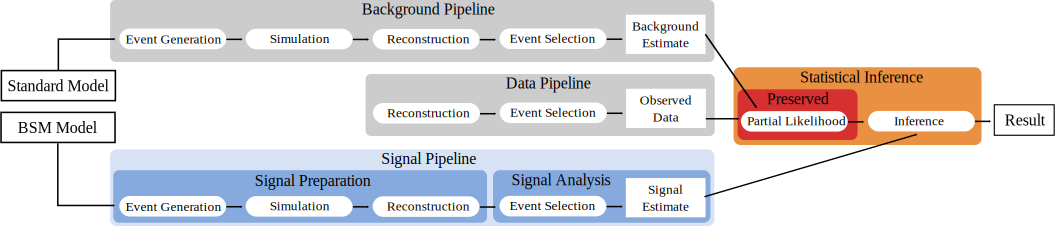
\includegraphics[width=\textwidth]{pipeline}
	\caption{Full analysis workflow including the three main processing pipelines for deriving background and signal estimates as well as observed data rates. The outputs of the three processing pipelines are combined into a likelihood forming the basis for statistical inference. Figure recreated from \reference\cite{ATL-PHYS-PUB-2019-032}.}
	\label{fig:pipeline_analysis}
\end{figure}

\subsection{Necessary ingredients}

As the event selection of an analysis is fixed, the background estimates and observed data in the targeted regions of interest do not change and can be archived in a suitable format. Reinterpreting a search in the light of a new signal model consequently only requires the signal pipeline in~\cref{fig:pipeline_analysis} to be run again, in order to derive the signal estimates that serve as input for the statistical inference. As the data and background processing pipelines shown in~\cref{fig:pipeline_analysis} only enter the statistical inference as estimated event rates, the volume of data that needs to be archived is significantly smaller than the original input data. As will be discussed in~\cref{sec:full_likelihood}, it has recently become technically possible to directly preserve the partial analysis likelihood built from the background estimates and observed data and including all details of the statistical model used for inference. Once the signal estimates are known, a new full analysis likelihood can be built, and the viability of the new signal model can be tested. 

Different approaches exist for deriving signal estimates. Manifestly the most precise approach involves running the original analysis using a different \gls{bsm} model. As this requires to preserve the entirety of the original software and workflows used in the analysis, this is arguably the most involved approach requiring knowledge of every detail of the analysis. \Cref{sec:recast_implementation} discusses an attempt at fully preserving the search for electroweakinos presented in this work. In many cases, the full precision of the original analysis pipeline is either not needed, or not accessible. 
As the full detector simulation requires access to the collaborations's detector description and is the most computationally expensive step in the signal pipeline, even when using fast simulations like \textsc{ATLFAST-II}, it is often approximated using simplified detector geometries and granularities. The most commonly used package for fast detector simulation outside of the collaboration is \textsc{Delphes}~\cite{Delphes:2009tx}. Other packages like \eg \textsc{Rivet}~\cite{Rivet1:2010ar,Rivet2:2019stt} approximate the detector response using dedicated 4-vector smearing techniques, assuming that the detector response roughly factorises into the responses of single particles. Internally, ATLAS also uses a dedicated framework for 4-vector smearing techniques, used in scenarios where other fast simulation techniques are still too expensive. \Cref{sec:truth_smearing} discusses these dedicated smearing functions further.

Similarly to the detector simulation, the analysis-specific event selection is also routinely approximated using different approaches. A number of public tools aiming to reimplement approximations of the event selections of various \gls{bsm} searches are available. Prominent examples include \textsc{CheckMate}~\cite{Checkmate2:2016npn,Checkmate:2013wra} and \textsc{MadAnalysis}~\cite{MadAnalysis:2012fm}. ATLAS has internally maintained a similar catalogue of its \gls{susy} analyses and has published event selection snippets in C++ on \textsc{HEPData}~\cite{HEPData:2017ypu}. Recently, this package maintained by ATLAS, called \textsc{SimpleAnalysis}, has been made publicly available, allowing the C++ snippets published to be run outside the collaboration.

Instead of trying to estimate the signal rates of a new signal model using \gls{mc} simulation and (reimplemented) analysis event selections, some reinterpretation efforts like \eg \textsc{SModelS}~\cite{SModelS1:2013mwa,SModelS2:2017neo} use \textit{efficiency maps} encoding the selection efficiency of the analysis as a function of some of the analysis observables (typically the sparticle masses). Such efficiency maps are routinely published by the ATLAS \gls{susy} searches on \textsc{HEPData}, and allows for efficient reinterpretations as long as the signal efficiencies mostly depend on the signal kinematics and are largely independent from the specific details of the signal model~\cite{SModelS1:2013mwa}. For the analysis presented in the previous part of this work, the efficiency maps and further analysis data products are available at \reference\cite{HEPdata_1Lbb}. 

\section{Public full likelihood}\label{sec:full_likelihood}

The likelihood is arguably one of the most information-dense and thus valuable data products of an analysis. Without precise knowledge of the exact likelihood of the original analysis, approximations need to be made for the statistical inference \eg in terms of correlations between event rate estimates as well as the treatment of uncertainties. Recently, ATLAS has started to publish full analysis likelihoods built using the \textsc{HistFactory} \gls{pdf} template introduced in~\cref{ch:statistics}~\cite{ATL-PHYS-PUB-2019-029}. This extraordinary step towards more open and reproducible science has been praised by the theory community~\cite{REINP:2020pec} as it allows for considerably more trustful reinterpretations. This effort has been facilitated by the development of \texttt{pyhf} in conjunction with the introduction of a \texttt{JSON} specification fully describing the \textsc{HistFactory} template. As a pure-text format, the \texttt{JSON} likelihoods are human- and machine-readable, highly compressible and can easily be put under version control, all of which are properties that make them ideal for long-term preservation. 

The full likelihood (in \texttt{JSON} format) of the search for electroweakinos presented in the previous part of this work has been published~\cite{fullLH_1Lbb} and is not only heavily used in the following chapters, but also in various analysis reinterpretation and combination efforts currently ongoing in ATLAS. Several efforts outside of the ATLAS collaboration have already included the analysis likelihood into their reinterpretations, \eg \textsc{SModelS}~\cite{SModelS_pyhf:2020grj} and \textsc{MadAnalysis}~\cite{Goodsell:2020ddr,Fuks:2021wpe} both reporting significant precision improvements through the use of the full likelihood (as opposed to approximating the statistical model). Furthermore, the full likelihood of the search presented herein has recently been used to demonstrate the concept of scalable distributed statistical inference on \glspl{hpc}~\cite{Feickert:2021sua}. Through the \texttt{funcX} package~\cite{chard20funcx}, \texttt{pyhf} is used as a highly scalable function as a service to fit the entire signal grid of 125 signal points within $\SI{156}{\second}$ on 85 available worker nodes\footnote{Theses benchmarks use \texttt{pyhf}'s \textsc{NumPy} backend and \textsc{SciPy} optimiser, which does have a slower log-likelihood minimisation time than \eg \textsc{PyTorch} coupled with \textsc{SciPy}.}.

\section{Analysis preservation using containerised workflows}\label{sec:recast_implementation}




\textsc{Recast}, originally proposed in \reference\cite{RECAST_cranmer} and recently used within ATLAS in \eg \reference\cite{ATL-PHYS-PUB-2019-032}




 \begin{figure}
	\centering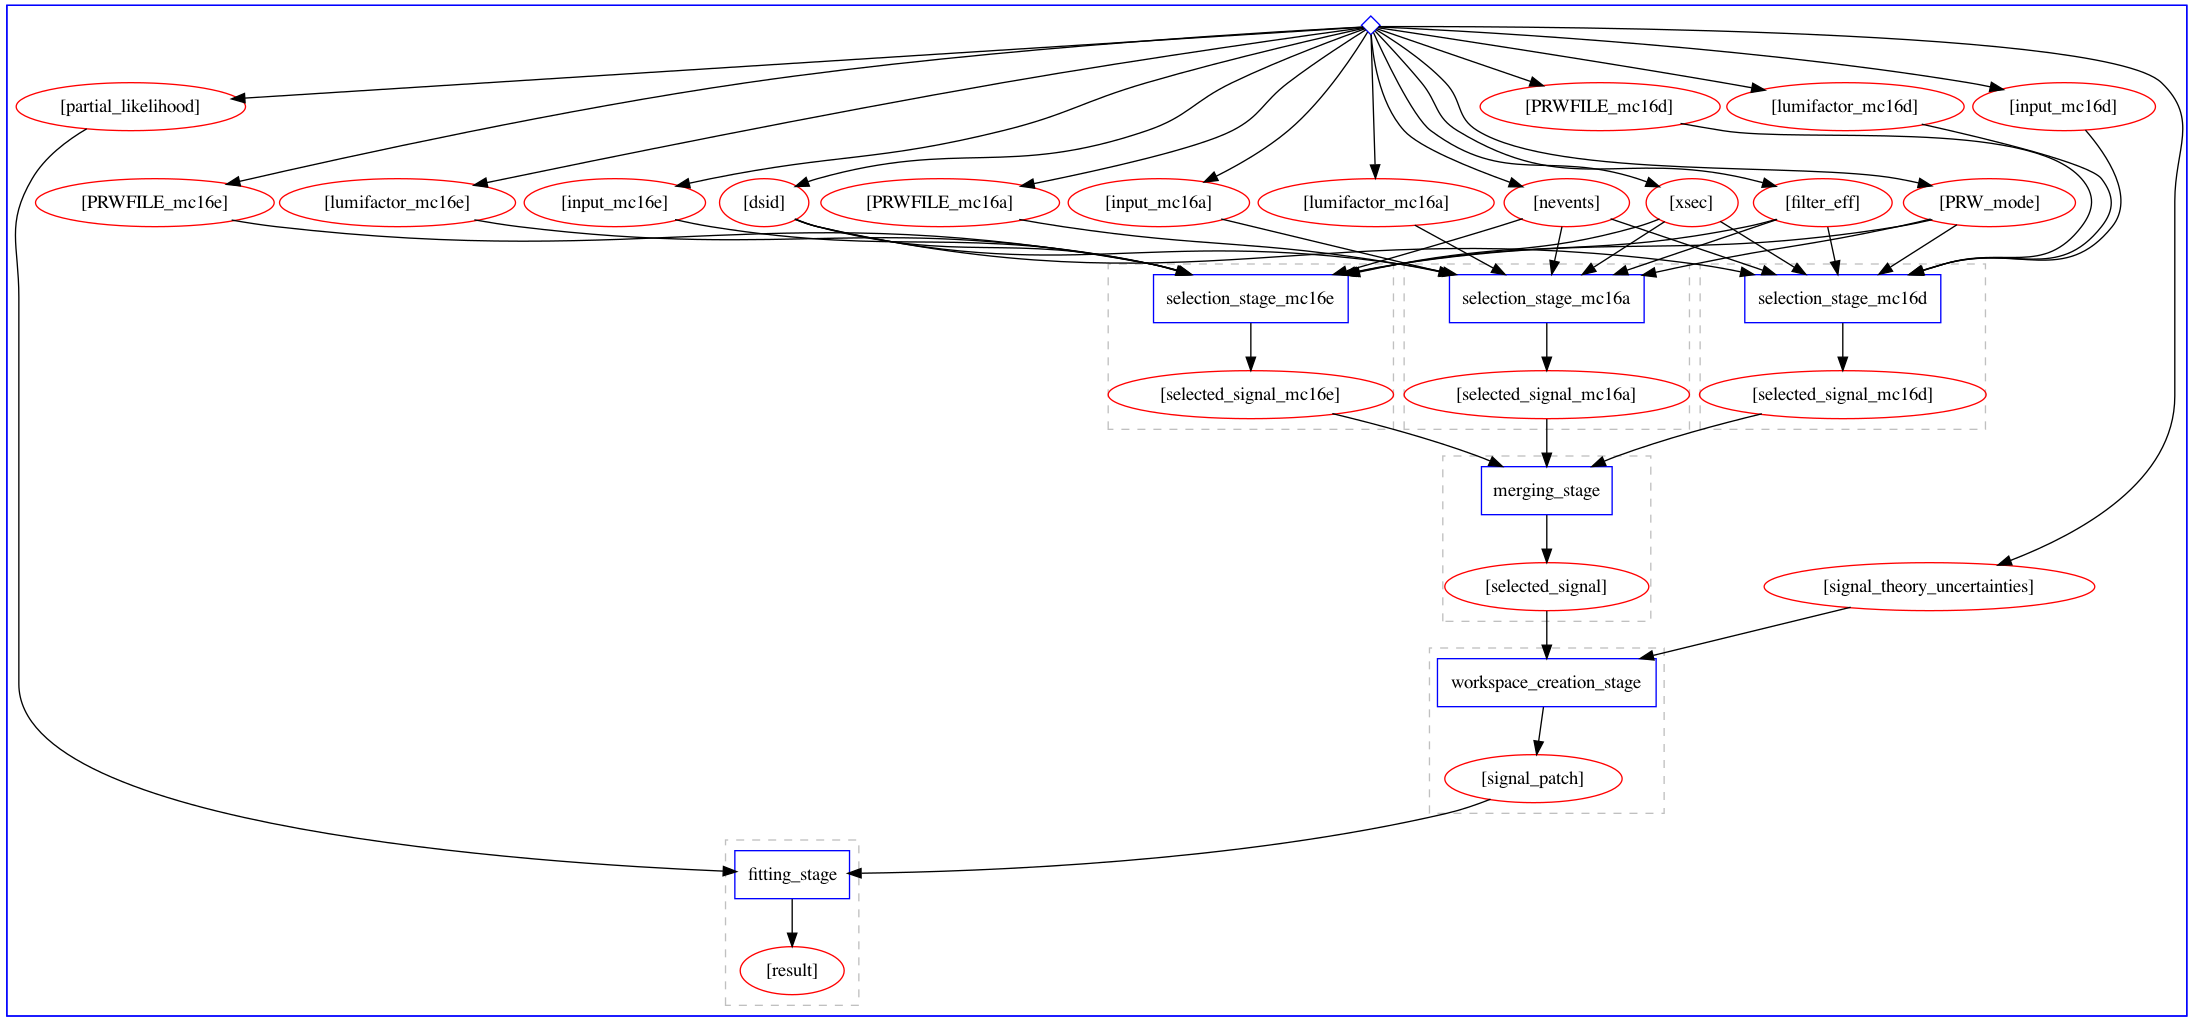
\includegraphics[width=\textwidth]{yadage_workflow_instance}
	\caption{Workflow}
	\label{fig:recast_workflow}
\end{figure}

